\documentclass[twoside,10pt]{article}
\usepackage[spanish, mexico]{babel}

%\usepackage[utf8x]{inputenc}

%\usepackage{hyperref}

\usepackage{subcaption}
\usepackage{multicol}
\usepackage{graphicx}
\usepackage{amssymb}
\usepackage{amsmath,amsfonts}
\usepackage{enumerate}
\usepackage{array}
%\usepackage{url}
%\usepackage{hyperref}

\usepackage{hyperref}
\usepackage{xcolor}
%\href{https://www.example.com}{[{\underline{\textcolor{blue}{link}}}]}

\setlength{\textheight}{23.5cm} \setlength{\evensidemargin}{0cm}
\setlength{\oddsidemargin}{0cm} \setlength{\topmargin}{-1.4cm}
\setlength{\textwidth}{16.5cm} \setlength{\parskip}{0.25cm}
\input xy
\xyoption{all}
%%-----------------------------------
\newtheorem{teo}{Teorema}[section]
\newtheorem{cor}[teo]{Corolario}
\newtheorem{lema}[teo]{Lema}
\newtheorem{prop}[teo]{Proposici\'on}
\newtheorem{defi}[teo]{Definici\'on}
\newtheorem{obs}[teo]{Observaci\'on}
\newtheorem{ejem}[teo]{Ejemplo}
\newtheorem{ejer}[teo]{Ejercicio}


\renewcommand{\Re}{\operatorname{Re}}
\newcommand{\C}{\mathbb{C}}
\newcommand{\R}{\mathbb{R}}
\newcommand{\Z}{\mathbb{Z}}
\newcommand{\Q}{\mathbb{Q}}


\numberwithin{equation}{section}
\renewcommand{\theequation}{\thesection.\arabic{equation}}
\newcommand{\Qed}{~\hfill$\square$}

%\pagestyle{myheadings} \markboth{Nombre corto del
%art\'iculo}{Jorge G., Andrik R., Osiel O., Christopher P., Jorge R., Marco N.M }


\setcounter{page}{2014} %P\'agina que se asigna una vez aceptado para publicaci\'on.

\begin{document}
\thispagestyle{plain} %En la primera p\'agina la numeraci\'on se despliega en la parte inferior.

\begin{flushleft}
\small{Abstraction \& Application {\bf volume} (year) $from \; page
\: x \; - \; to \; page \;y$} \hfill UADY

\includegraphics[angle=0,width=0.06\linewidth]{UADY.jpg} %Escudo de la UADY, el cual puede ser sustituido por el escudo de la instituci\'on de adscripci\'on del autor para correspondencia.
\end{flushleft}

\bigskip

\begin{center}

{\bf{\Large Implementación de interfaz gráfica en PyQt5 referente a Linear Classification Loss Visualization}}

\vspace{0.2cm}

{\large {$^a$Jorge Guevara García, $^b$José Andrik Martínez Rodriguez, $^c$Osiel Alejandro Ordoñez Cruz, $^d$Christopher Emmanuel Pérez Duque, $^e$Jorge Jhovan Rodriguez Moreno, $^f$Marco Aurelio Nuño Maganda.} }

\vspace{0.2cm}

$^a$Universidad Politécnica de Victoria. Avenida Nuevas Tecnologías 5902, Parque Científico y Tecnológico de Tamulipas, Victoria, Tamulipas, 87138, México.

\medskip

\{2030192, 2030152, 2030023, 2030358, 2030295, mnunom\}@upv.edu.mx.

\end{center}

%$\hspace{3.6mm}$\begin{minipage}[t][2cm][s]{14.72cm} {\small
%\begin{center} {\bf Abstract} \end{center}
%$\hspace{2.5mm}$ Aqui va el resumen en ingl\'{e}s.}
%\end{minipage}

\renewcommand{\abstractname}{Abstract}
\begin{abstract}
This project focuses on the implementation and evaluation of linear classification algorithms, as well as the visualization of loss. The implementation includes a graphical user interface developed in Python, utilizing libraries such as PyQt5 for interactive GUI components and Matplotlib for data visualization. The algorithm itself is based on a classification model that utilizes weights and biases to separate data points into different classes. The implementation allows for a deeper understanding of the algorithm's functionality and its visual representation through the graphical interface.
\end{abstract}

\renewcommand{\abstractname}{Resumen}
\begin{abstract}
Este proyecto se centra en la implementación y evaluación de algoritmos de clasificación lineal, así como en la visualización de la pérdida. La implementación incluye una interfaz gráfica de usuario desarrollada en Python, utilizando bibliotecas como PyQt5 para componentes interactivos de la interfaz gráfica y Matplotlib para la visualización de datos. El algoritmo en sí se basa en un modelo de clasificación que utiliza pesos y sesgos para separar los puntos de datos en diferentes clases. La implementación permite comprender mejor la funcionalidad del algoritmo y su representación visual a través de la interfaz gráfica.
\end{abstract}

%$\underline{\hspace{3.5cm}}$

$\underline{ \ \ \ \ \ \ \ \ \ \ \  \ \ \ \ \ \ \ \ \ \ \ \ \ \ \ \
\ }$

{\footnotesize $Keywords$ $and$ $phrases:$ Linear classification,
Loss visualization, Multiclass Support Vector Machine (SVM), Training data, Classification model}


$\overline{ \ \ \ \ \ \ \ \ \ \ \  \ \ \ \ \ \ \ \ \ \ \ \ \ \ \ \ \
}$
\section{Introducción}

En este tema, exploraremos la Linear classification Loss Visualization (Visualización de la Pérdida de Clasificación Lineal). En el campo del aprendizaje automático y la visión por computadora, la clasificación lineal es una técnica ampliamente utilizada para asignar etiquetas a los datos. La pérdida de clasificación lineal es una medida de cuán bien se ajustan los datos a un modelo lineal y se utiliza para ajustar los parámetros del modelo durante el entrenamiento.

La visualización de la pérdida de clasificación lineal es una herramienta importante para comprender y analizar el rendimiento del modelo. Permite identificar patrones en los datos que pueden afectar la precisión de la clasificación y proporciona información sobre cómo ajustar los parámetros del modelo para mejorar el rendimiento. La visualización de la pérdida de clasificación lineal es para los científicos de datos, los ingenieros de aprendizaje automático y los investigadores que trabajan en problemas de clasificación. Proporciona información crucial para comprender y mejorar los modelos de clasificación lineal y puede conducir a avances significativos en el rendimiento y la precisión de los sistemas de clasificación.

En este contexto, exploraremos y analizaremos diferentes técnicas y métodos para visualizar la pérdida de clasificación lineal. Utilizaremos gráficos y diagramas para representar la relación entre los datos de entrada y la pérdida de clasificación, lo que nos permitirá identificar posibles áreas problemáticas y realizar ajustes en el modelo.

\section{Linear classification Loss Visualization}

La clasificación lineal es una técnica ampliamente utilizada para asignar etiquetas a los datos en diversos problemas de clasificación. La pérdida de clasificación lineal es una medida de cuán bien se ajustan los datos a un modelo lineal y se utiliza para ajustar los parámetros del modelo durante el entrenamiento. En esta sección, exploraremos la visualización de la pérdida de clasificación lineal y su importancia en el análisis y mejora de modelos de clasificación lineal.

La visualización de la pérdida de clasificación lineal es una herramienta clave para comprender y analizar el rendimiento de un modelo de clasificación lineal. Permite identificar patrones en los datos que pueden afectar la precisión de la clasificación y proporciona información sobre cómo ajustar los parámetros del modelo para mejorar su rendimiento. La visualización de la pérdida de clasificación lineal es especialmente útil para científicos de datos, ingenieros de aprendizaje automático e investigadores que trabajan en problemas de clasificación.

La pérdida de clasificación lineal se calcula utilizando una función de pérdida, como la pérdida de Máquina de Vectores de Soporte Multiclase (Multiclass Support Vector Machine, SVM). Esta función de pérdida compara las puntuaciones de clase predichas por el modelo con las etiquetas reales de los datos de entrenamiento y mide la discrepancia entre ellas. Cuanto mayor sea la pérdida, peor será el ajuste del modelo a los datos.

La visualización de la pérdida de clasificación lineal implica representar gráficamente la relación entre la pérdida y otros parámetros o características relevantes. Por ejemplo, se puede visualizar la pérdida en función del número de iteraciones de entrenamiento para observar cómo disminuye a medida que el modelo se ajusta mejor a los datos. También se pueden crear gráficos que muestren la pérdida en función de diferentes hiperparámetros del modelo, como el tamaño del paso de aprendizaje (learning rate) o la regularización. Estas visualizaciones pueden proporcionar información valiosa sobre cómo ajustar estos parámetros para obtener un mejor rendimiento del modelo.

A continuación, se presentan algunas ecuaciones de ejemplo que muestran cómo se calcula la pérdida de clasificación lineal utilizando la pérdida de SVM multiclase:

Dado un ejemplo de entrenamiento $i$ con píxeles $x_i$ y etiqueta $y_i$, la función de puntuación calcula un vector de puntuaciones de clase $s$:
\begin{equation}
s = f(x_i, W)
\end{equation}

La pérdida de SVM multiclase para este ejemplo se calcula como:
\begin{equation}
L_i = \sum_{j \neq y_i} \max(0, s_j - s_{y_i} + \Delta)
\end{equation}

donde $s_j$ es la puntuación para la clase $j$, $s_{y_i}$ es la puntuación para la clase correcta $y_i$, y $\Delta$ es un margen fijo que define la diferencia mínima deseada entre las puntuaciones de la clase correcta e incorrecta.

La visualización de la pérdida de clasificación lineal puede incluir gráficos de líneas, gráficos de dispersión o diagramas de contorno para representar la relación entre la pérdida y los parámetros del modelo. Estas visualizaciones ayudan a los investigadores y practicantes a comprender cómo el modelo se ajusta a los datos y a identificar posibles áreas problemáticas que requieren mejoras.

Se concluye esta sección añadiendo que la visualización de la pérdida de clasificación lineal es una herramienta esencial para analizar y mejorar los modelos de clasificación lineal. Permite comprender cómo se ajustan los datos al modelo y proporciona información valiosa sobre cómo ajustar los parámetros para lograr un mejor rendimiento. La visualización de la pérdida de clasificación lineal es una práctica común en el campo del aprendizaje automático y la visión por computadora, y puede conducir a avances significativos en la precisión y eficacia de los sistemas de clasificación lineal.




\section{Marco teórico}

La visualización de la pérdida de clasificación lineal es un tema importante en el campo del aprendizaje automático y se refiere a la representación gráfica de la función de pérdida utilizada en clasificadores lineales.
La visualización de la pérdida en la clasificación lineal es un campo de estudio que se enfoca en comprender y representar de manera gráfica la función de pérdida utilizada en los algoritmos de clasificación lineal. Esta visualización proporciona una herramienta poderosa para analizar y evaluar el rendimiento de los modelos de clasificación lineal, así como para comprender la convergencia y los desafíos asociados con la optimización de los hiperplanos de decisión. \cite{Linear-Classification-Loss}

La clasificación lineal es un enfoque común en el aprendizaje automático supervisado, donde el objetivo es separar los datos en diferentes clases utilizando un hiperplano de decisión. La función de pérdida, también conocida como función de costo, es una medida que evalúa qué tan bien se ajusta el modelo a los datos y se utiliza para optimizar los parámetros del modelo.\cite{Linear-Classification}

Los puntajes de clase para los clasificadores lineales se calculan como $f(x_i; W, b) = W x_i + b$, donde los parámetros consisten en los pesos W y los sesgos b. Los datos son $x_i$ con etiquetas $y_i$. En esta demostración, los puntos de datos $x_i$ son de 2 dimensiones y hay 3 clases, por lo que la matriz de pesos es de tamaño $[3 x 2]$ y el vector de sesgos es de tamaño [3 x 1]. La función de pérdida multiclase se puede formular de muchas maneras. El valor predeterminado en esta demostración es una SVM que sigue [Weston y Watkins 1999]. Denotando f como el vector [3 x 1] que contiene los puntajes de clase, la pérdida tiene la forma:
\begin{center}
    $L = \frac{1}{N} \sum_i \sum_{j \neq y_i} \max(0, f_j - f_{y_i} + 1) + \lambda \sum_k\sum_l W_{k,l}^2$
\end{center}
Donde $N$ es el número de ejemplos y $\lambda$ es un hiperparámetro que controla la fuerza de la penalización de regularización $L2 R(W) = \sum_k\sum_l W_{k,l}^2$. En la parte inferior derecha de esta demostración, también puedes cambiar a diferentes formulaciones para la SVM multiclase, incluyendo Uno contra Todos (OVA) donde se entrena una SVM binaria separada para cada clase de forma independiente (vs. las otras clases etiquetadas como negativas), y la SVM Estructurada que maximiza el margen entre el puntaje correcto y el puntaje de la clase competidora más alta. También puedes elegir utilizar la pérdida de entropía cruzada que se utiliza en el clasificador Softmax. \cite{Linear-Classification-Loss}

%En el marco conceptual de la visualización de la pérdida en la clasificación lineal, se pueden identificar varios elementos clave. Como los que se presentan a continuación:
%\begin{enumerate}
%    \item \textbf{Clasificación lineal:} La clasificación lineal es una técnica utilizada en el aprendizaje automático para asignar objetos a diferentes clases en función de una línea de decisión lineal. Los clasificadores lineales se basan en la suposición de que los datos se pueden separar mediante una combinación lineal de características.
%    \item \textbf{Función de pérdida:} La función de pérdida es una medida que cuantifica la discrepancia entre las etiquetas de clase predichas y las etiquetas de clase reales. En el contexto de la clasificación lineal, la función de pérdida se utiliza para evaluar qué tan bien el clasificador está realizando la tarea de clasificación.
%    \item \textbf{Visualización de la pérdida de clasificación lineal:} La visualización de la pérdida de clasificación lineal implica representar gráficamente la función de pérdida en función de diferentes parámetros o variables. Esto puede ayudar a comprender el comportamiento del clasificador y el impacto de los diferentes parámetros en el rendimiento de la clasificación.
%    \item \textbf{Tipos de funciones de pérdida:} En los clasificadores lineales, se utilizan diferentes funciones de pérdida para medir la discrepancia entre las etiquetas de clase predichas y las etiquetas de clase reales. Algunos ejemplos comunes de funciones de pérdida incluyen:
 %   \begin{itemize}
%        \item Pérdida de bisagra (hinge loss): Es una función de pérdida utilizada en clasificadores de margen máximo, como las máquinas de vectores de soporte (SVM). La pérdida de bisagra penaliza las predicciones incorrectas y busca maximizar el margen entre las clases.
%        \item Pérdida softmax: Es una función de pérdida utilizada en la regresión logística multinomial. La pérdida softmax mide la probabilidad de cada clase y busca minimizar la entropía cruzada entre las distribuciones de probabilidad predichas y las distribuciones de probabilidad reales.
%    \end{itemize}
%\item \textbf{Herramientas y recursos:} Existen diversas herramientas y recursos disponibles para visualizar la pérdida de clasificación lineal. Algunas de estas herramientas incluyen bibliotecas de visualización de datos en Python, como Matplotlib, que permiten representar gráficamente la función de pérdida en función de diferentes variables.
%\end{enumerate}
En resumen, la visualización de la pérdida de clasificación lineal es una técnica importante en el aprendizaje automático que permite comprender y analizar el rendimiento de los clasificadores lineales. Al representar gráficamente la función de pérdida, se pueden obtener ideas sobre el comportamiento del clasificador y optimizar los parámetros para mejorar la precisión de la clasificación.



\section{Implementación y Resultados}
La implementación de este proyecto es un paso crucial para analizar y evaluar el rendimiento de los algoritmos de clasificación lineal, así como para explorar visualmente la forma en que se produce la pérdida.

En primer lugar, presentaremos una descripción general de los métodos y enfoques utilizados en la implementación. Discutiremos las bibliotecas y herramientas utilizadas, así como los lenguajes de programación específicos que se emplearon para desarrollar este sistema. Además, se proporcionará información sobre el entorno de desarrollo y los requisitos técnicos necesarios para ejecutar la implementación.

La implementación de este proyecto consta de una interfaz gráfica de usuario desarrollada en el lenguaje de programación Python utilizando las bibliotecas gráficas como PyQt5 que  proporciona componentes y herramientas para desarrollar interfaces gráficas de usuario. Se utiliza para construir la interfaz gráfica interactiva de la aplicación y Matplotlib que ayuda a la visualización de datos en Python. Se utiliza para generar gráficos y visualizar los datos de entrenamiento, así como las líneas de clasificación del algoritmo.

El algoritmo implementado se basa en un modelo de clasificación que utiliza pesos y sesgos para separar los puntos de datos en diferentes clases. A continuación se presenta una explicación del funcionamiento del algoritmo y su interacción con la interfaz gráfica:

\begin{enumerate}
    \item \textbf{Inicialización:} Al iniciar la aplicación, se inicializan los datos, los pesos y los sesgos del modelo. Los datos se representan como una matriz bidimensional de coordenadas (X) y una matriz de etiquetas de clase (y). Los pesos y sesgos se inicializan como matrices de ceros.
    \item \textbf{Interfaz gráfica:} La interfaz gráfica se compone de varios componentes, incluyendo controles deslizantes, botones y etiquetas. Estos componentes permiten al usuario interactuar con el modelo y ajustar los parámetros.
    \item \textbf{Ajuste de parámetros:} El usuario puede ajustar los pesos y sesgos del modelo utilizando los botones de aumento y disminución correspondientes a cada parámetro. Al hacer clic en estos botones, se actualizan los valores de los parámetros y se recalculan las puntuaciones y la pérdida del modelo.
    \item \textbf{Cálculo de puntuaciones y pérdida:} Se calculan las puntuaciones del modelo para cada ejemplo utilizando los pesos y sesgos actuales. Las puntuaciones se obtienen multiplicando las características de los ejemplos por los pesos, sumando los sesgos y aplicando una función de activación softmax. A continuación, se calcula la pérdida del modelo utilizando la entropía cruzada negativa. La pérdida se muestra en la interfaz gráfica.
    \item \textbf{Cálculo de gradientes:} Se calculan los gradientes de la función de pérdida con respecto a los pesos y sesgos utilizando el método de retropropagación. Los gradientes se utilizan posteriormente para actualizar los parámetros del modelo durante su aprendizaje.
    \item \textbf{Actualización de parámetros:} El usuario puede actualizar los parámetros del modelo de dos formas. Primero, puede hacer clic en el botón ``Single parameter update" para actualizar un solo parámetro a la vez. Segundo, puede activar el botón ``Start repeated update" para iniciar una actualización periódica de los parámetros utilizando un temporizador. El tamaño de paso para las actualizaciones se puede ajustar mediante un control deslizante.
    \item \textbf{Visualización:} Se utiliza Matplotlib para generar un gráfico interactivo que muestra los datos y las líneas de clasificación del modelo. El gráfico se actualiza automáticamente cuando se realizan cambios en los parámetros del modelo.
\end{enumerate}

\subsection{Estructura del programa:}
El programa de clasificación de puntos se compone de varias clases que trabajan en conjunto para permitir la interacción con puntos en un espacio bidimensional y realizar clasificaciones basadas en sus coordenadas. Donde las clases codificadas y sus funcionalidades son las siguientes:
\begin{enumerate}
    \item \textbf{DrawWidget:} Esta clase representa un widget en el que se dibujan puntos. Los puntos se definen como instancias de la clase \textbf{Point}, que contiene coordenadas (x, y) y una clase asociada. El widget permite mover los puntos cuando se hace clic y arrastra el mouse sobre ellos. La función paintEvent se encarga de dibujar los puntos en el widget.
    \item \textbf{Window:} Esta clase representa la ventana principal de la aplicación. Se encarga de gestionar la interfaz gráfica, incluyendo la disposición de los elementos y la interacción con los botones y sliders. Las funciones más importantes en esta clase son:
    \begin{itemize}
        \item \textbf{actualizarCoordenadas:} Actualiza las coordenadas de los puntos en base a las posiciones actuales en el DrawWidget.
        \item \textbf{calcularS:} Calcula las puntuaciones (s) para cada punto en base a los pesos y las coordenadas de los puntos.
        \item \textbf{calcular\_perdida:} Calcula la pérdida para cada punto en base a las puntuaciones y las clases reales. También calcula la pérdida media, la pérdida de regularización y la pérdida total.
        \item \textbf{calcular\_gradientes:} Calcula los gradientes de la función de pérdida con respecto a los pesos y los sesgos.
        \item \textbf{update\_parameters:} Actualiza los pesos y los sesgos utilizando los gradientes y el tamaño de paso. También recalcula las puntuaciones, la pérdida y los gradientes después de la actualización.
        \item \textbf{plot:} Grafica los puntos y las regiones de clasificación utilizando Matplotlib.
    \end{itemize}
\end{enumerate}

%Apartado de resultados
En este apartado, presentaremos los resultados obtenidos tras la implementación del proyecto, donde se analizó y evaluó el rendimiento de los algoritmos de clasificación lineal. Además, exploramos visualmente la forma en que se producen los resultados en este contexto. A continuación, detallaremos los hallazgos más relevantes.

En primer lugar, describiremos la implementación y los enfoques utilizados en este proyecto. Se desarrolló una interfaz gráfica de usuario utilizando el lenguaje de programación Python y diversas bibliotecas gráficas como PyQt5 y Matplotlib. Estas herramientas nos permitieron crear una interfaz interactiva que facilita la interacción con el modelo de clasificación y la visualización de los datos y las líneas de clasificación generadas.

El algoritmo implementado se basa en un modelo de clasificación lineal que utiliza pesos y sesgos para separar los puntos de datos en diferentes clases. Durante la implementación, se inicializaron los datos de entrenamiento, los pesos y los sesgos del modelo. Luego, la interfaz gráfica permitió interactuar con los parámetros del modelo y calcular las puntuaciones, la pérdida y los gradientes correspondientes. Además, se agregaron botones para mejorar la facilidad de entendimiento y rendimiento del sistema.

En los resultados obtenidos, se observó que el modelo de clasificación lineal logra separar efectivamente los puntos de datos en diferentes clases. Al ajustar los pesos y sesgos a través de la interfaz gráfica, pudimos visualizar cómo las líneas de clasificación se adaptaban a los cambios en los parámetros del modelo. Además, al analizar la pérdida del modelo, observamos una disminución a medida que se actualizaban los parámetros utilizando la retropropagación y los gradientes calculados. Esta disminución en la pérdida indica que el modelo está aprendiendo y mejorando su capacidad de clasificación.

En términos de visualización, la interfaz gráfica junto con Matplotlib nos permitió representar gráficamente los puntos de datos, así como las regiones de clasificación generadas por el modelo. Esto nos proporcionó una comprensión visual clara de cómo el algoritmo de clasificación lineal divide el espacio bidimensional en clases separadas. A continuación, presentaremos un análisis detallado de los resultados obtenidos para una mejor comprensión.


%Primera imagen interfaz
La primera imagen que presentamos es una captura de pantalla de la interfaz de la aplicación desarrollada para este proyecto de investigación.
La imagen muestra una vista general de la interfaz, donde se pueden apreciar diferentes componentes que permiten la interacción con el modelo de clasificación lineal implementado y la visualización de los datos. 
\begin{enumerate}
        \item Zona de visualización: En la parte izquierda de la interfaz, se encuentran dos áreas de visualización donde se muestran los puntos de datos y las líneas de clasificación generadas por el modelo. Esta zona proporciona una representación gráfica clara de cómo se están clasificando los datos.
        \item Botones de pesos: En el centro de la interfaz, se encuentran los botones para el manejo que permiten ajustar los parámetros del modelo. Estos controles brindan al usuario la capacidad de modificar los pesos para observar cómo afectan las líneas de clasificación y la precisión del modelo.
        \item Botones de interacción: En la parte inferior de la interfaz, se encuentran una serie de botones que mejoran la interacción con la aplicación. Estos botones permiten al usuario realizar acciones como ajustar los parámetros de forma individual o iniciar una actualización periódica de los parámetros utilizando un temporizador, pausar de manera inmediata la ejecución y inhabilitar la graficación.
        \item Resultados e información adicional: En la parte superior derecha de la interfaz, se pueden mostrar resultados y métricas relevantes, como la precisión del modelo, la pérdida calculada y otros datos estadísticos. 

        %\begin{figure}[ht]
         %   \centering
          %  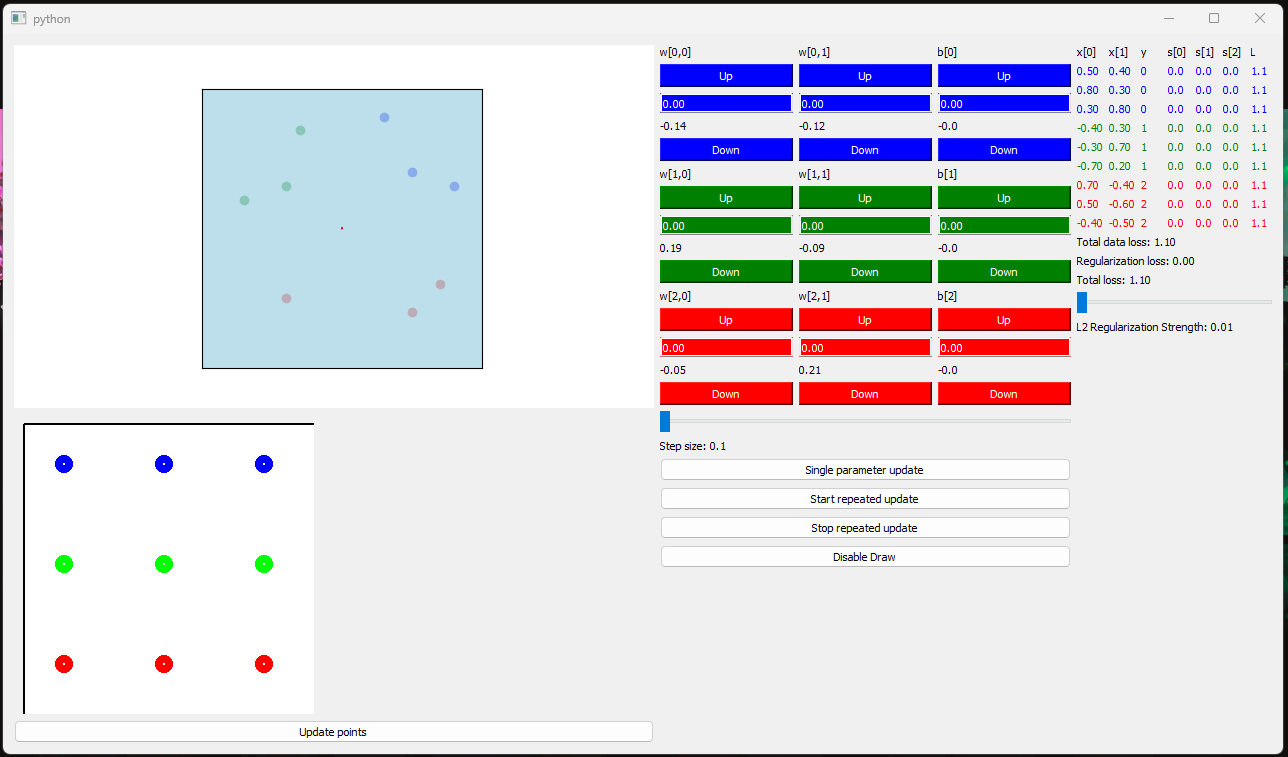
\includegraphics[width=0.5\linewidth]{grafics/img-001.png}
           % \caption{Interfaz de la aplicación.}
            %\label{fig:after-label}
        %\end{figure}
\end{enumerate}


La segunda imagen que presentamos muestra una captura de pantalla de la interfaz de la aplicación en acción, donde se realiza el movimiento de los puntos de datos en la parte inferior izquierda. En esta imagen, podemos observar cómo los puntos de datos se han movido en el área designada mediante la interacción directa con los puntos que se encuentran en el área, los usuarios pueden explorar diferentes escenarios y observar cómo se modifican las líneas de clasificación en tiempo real. Esto facilita la comprensión de cómo pequeños cambios en la posición de los puntos pueden afectar la precisión y el rendimiento del modelo.
%Seg imagen 
%\begin{figure}[ht]
    %\centering
    %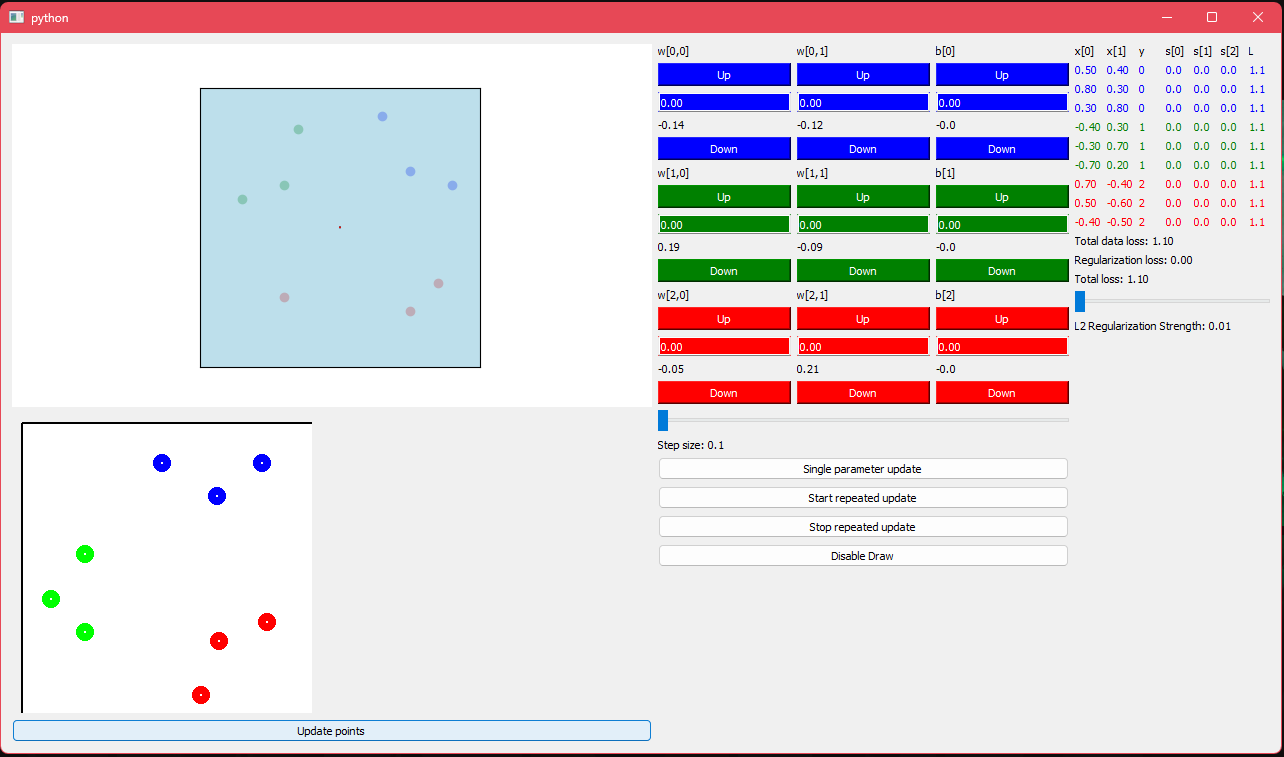
\includegraphics[width=0.5\linewidth]{grafics/img-002.png}
    %\caption{Ubicación de puntos en coordenadas diferentes.}
    %\label{fig:after-label2}
%\end{figure}



\begin{figure}[ht]
    \centering
    \subfloat[Interfaz de la aplicación.\label{fig:1}]{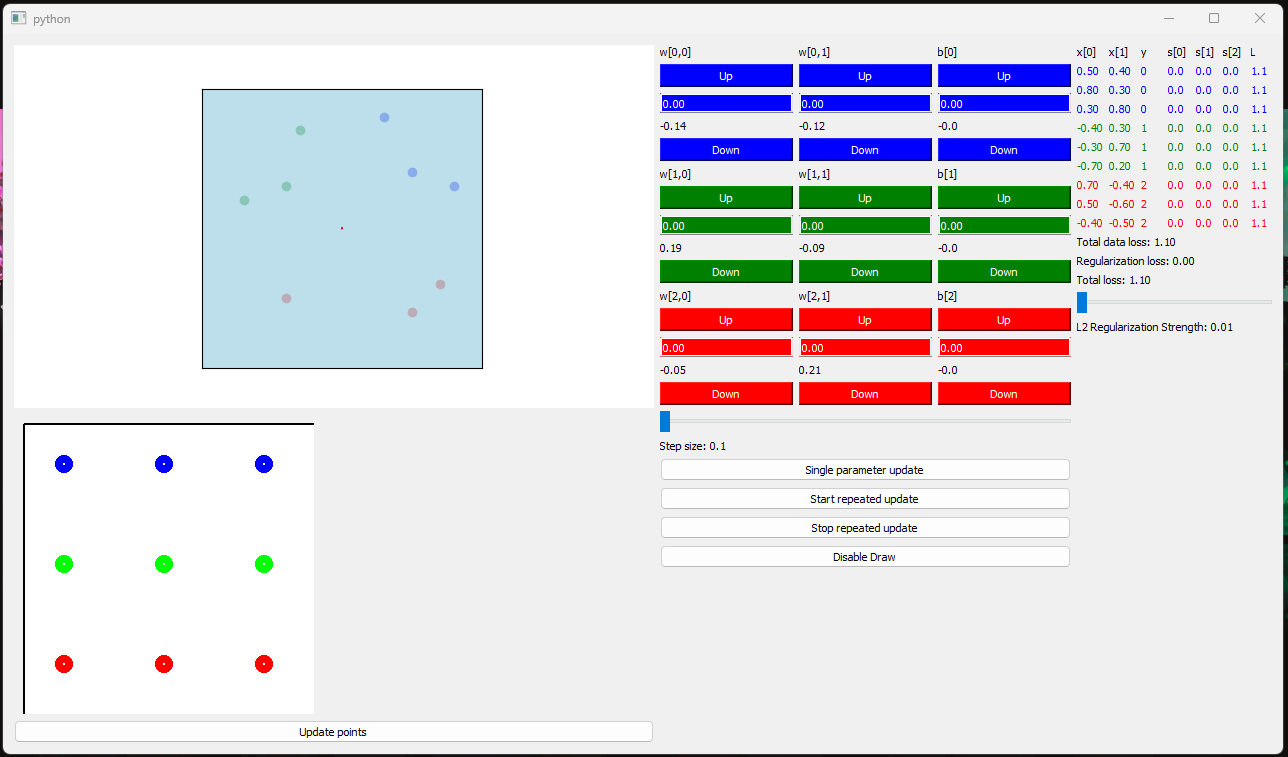
\includegraphics[width=0.4 \columnwidth]{grafics/img-001.png}}
    \hspace{1cm}
    \subfloat[Ubicación de puntos en coordenadas diferentes.\label{fig:2}]{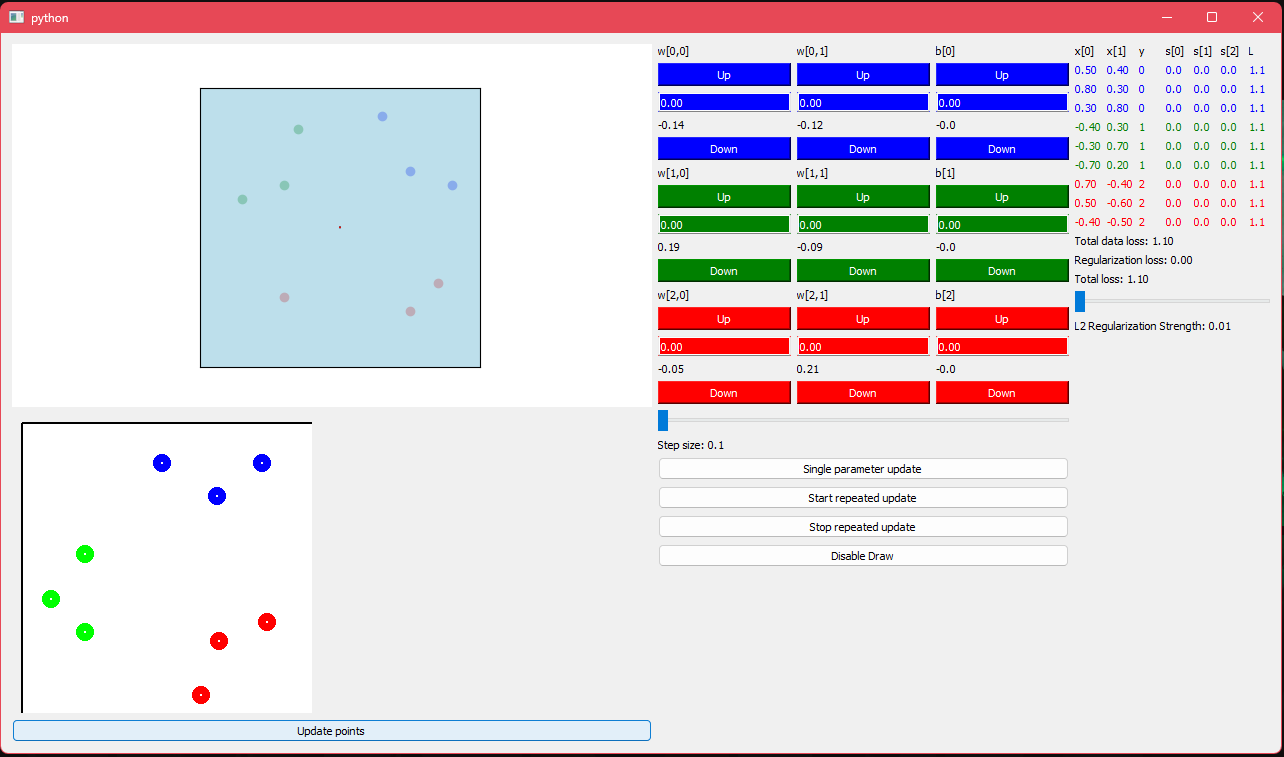
\includegraphics[width=0.4\columnwidth]{grafics/img-002.png}}
    \caption{Figuras 1 y 2}
\end{figure}

La tercera imagen que presentamos es una captura de pantalla de la interfaz de la aplicación después de hacer uso del botón Update Points. Esta funcionalidad permite actualizar la ubicación de los puntos de datos en el gráfico principal de la interfaz.

En la imagen, podemos observar cómo los puntos de datos en el área designada se han colocado nuevamente en el gráfico principal, reemplazando los puntos anteriores. Esta capacidad de actualización de los puntos de datos ofrece una forma conveniente de examinar diferentes configuraciones de los datos y su impacto en la clasificación realizada por el modelo de clasificación lineal.

Al utilizar el botón Update Points, los usuarios pueden generar de forma rápida y sencilla nuevos conjuntos de datos y visualizar cómo se clasifican bajo el modelo implementado. Esto facilita la exploración de diferentes escenarios y evaluación del desempeño del modelo en diversas configuraciones de datos.
%Ter imagen 



En la cuarta imagen presentada en este artículo, mostramos una captura de pantalla de la interfaz de la aplicación después de hacer uso del botón Single Parameter Update. Esta función permite realizar una actualización individual de el proceso de clasificación lineal.

En la imagen, podemos observar cómo los datos se han actualizado y la gráfica principal se ha coloreado con tonos de verde, rojo y azul. Estos colores representan la clasificación de los puntos de datos según su ubicación en relación con el valor actualizado del parámetro específico.

La coloración en verde, rojo y azul en la gráfica principal permite identificar rápidamente cómo se distribuyen los puntos de datos en relación con el parámetro actualizado. Los puntos clasificados en verde representan una clase específica, mientras que los puntos en rojo y azul corresponden a otras dos clases diferentes.
%4ta imagen
\begin{figure}
    \centering
    \subfloat[Update de puntos en la gráfica principal.\label{fig:3}]{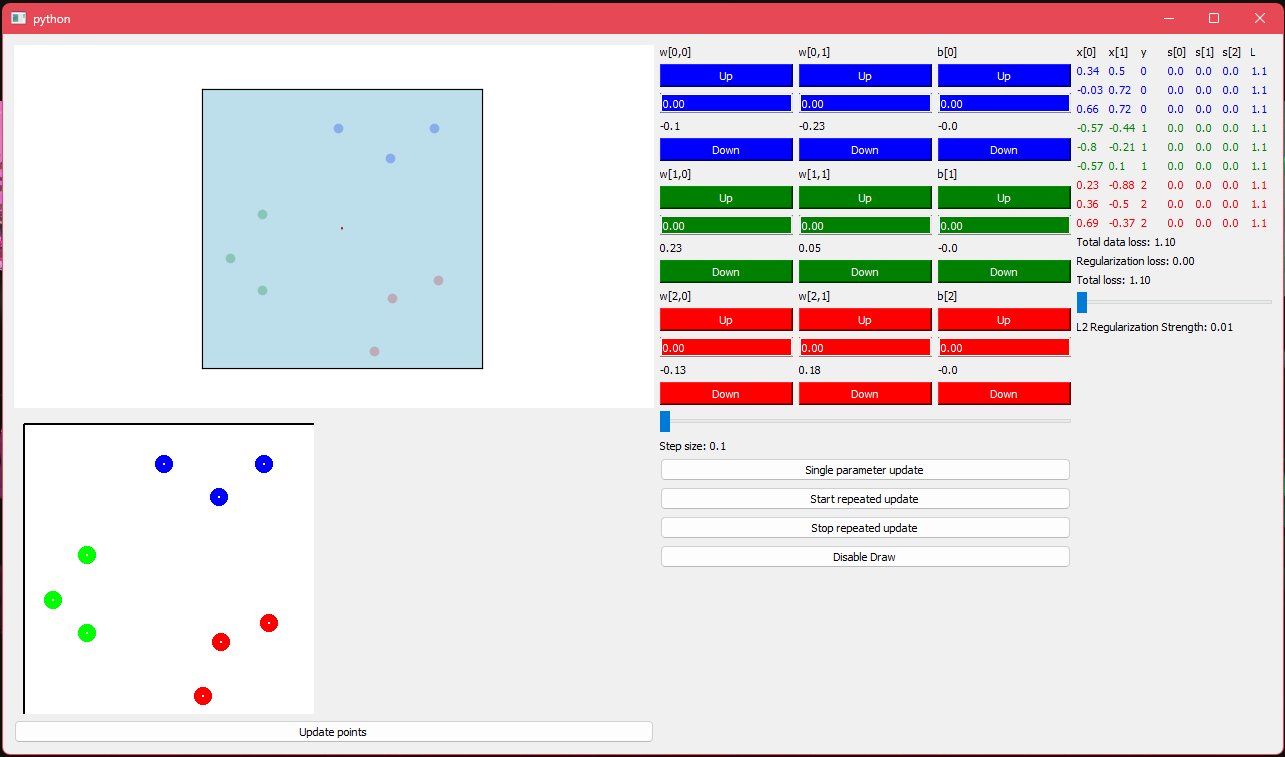
\includegraphics[width=0.4 \columnwidth]{grafics/img-003.png}}
    \hspace{1cm}
    \subfloat[Uso del bóton \textit{single parameter update}\label{fig:4}]{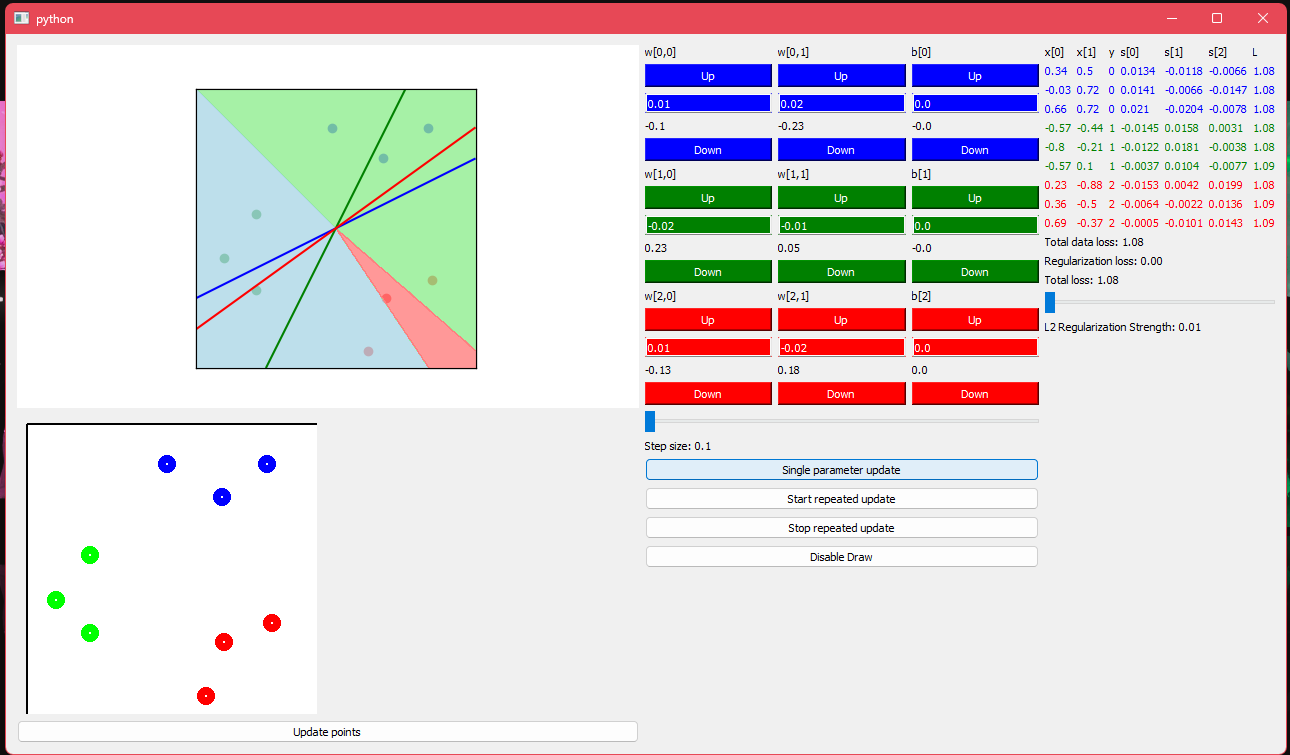
\includegraphics[width=0.4\columnwidth]{grafics/img-004.png}}
    \caption{Figuras 3 y 4}
\end{figure}







%5ta imagen 
En la quinta imagen, mostramos una captura de pantalla de la interfaz de la aplicación después de hacer uso del botón Disable Draw. Esta funcionalidad permite desactivar únicamente la representación gráfica en el gráfico principal, mientras que las métricas y los valores continúan actualizándose.

En la imagen, podemos observar que el área gráfica se encuentra en un estado inactivo, sin actualizar las líneas de clasificación y los puntos de datos. Sin embargo, las métricas relevantes, como la precisión del modelo y la pérdida calculada, siguen actualizándose y se muestran en la interfaz.

Al hacer clic en el botón Disable Draw, se desactiva la actualización visual en el gráfico principal y para volver a reactiva solo es necesario volver a dar clic en el bóton. Esto puede ser útil en situaciones donde se desea centrar la atención en las métricas y los valores numéricos sin distracciones visuales.

%6ta imagen
La sexta imagen que presentamos en este artículo muestra una captura de pantalla de la interfaz de la aplicación después de hacer uso del botón Start Repeated Update. Esta función permite realizar actualizaciones periódicas de las métricas, los valores y la gráfica principal de manera continua.

En la imagen, podemos observar cómo las métricas, los valores y la gráfica principal se actualizan de forma constante y simultánea. Esto se refleja en los cambios dinámicos de las líneas de clasificación, los puntos de datos y las métricas en tiempo real.

Al hacer clic en el botón Start Repeated Update, se inicia un proceso de actualización repetida que permite observar cómo el modelo de clasificación lineal evoluciona y se adapta a medida que se modifican los parámetros.

Esta funcionalidad proporciona una forma dinámica de monitorear el rendimiento y la precisión del modelo a medida que se actualizan las métricas y se genera la gráfica principal. Permite una visualización continua y en tiempo real de la clasificación de los puntos de datos y el impacto de los cambios en los parámetros.
%6ta imagen 
\begin{figure}[ht]
    \centering
    \subfloat[Deshabilitado la graficación en tiempo real.\label{fig:5}]{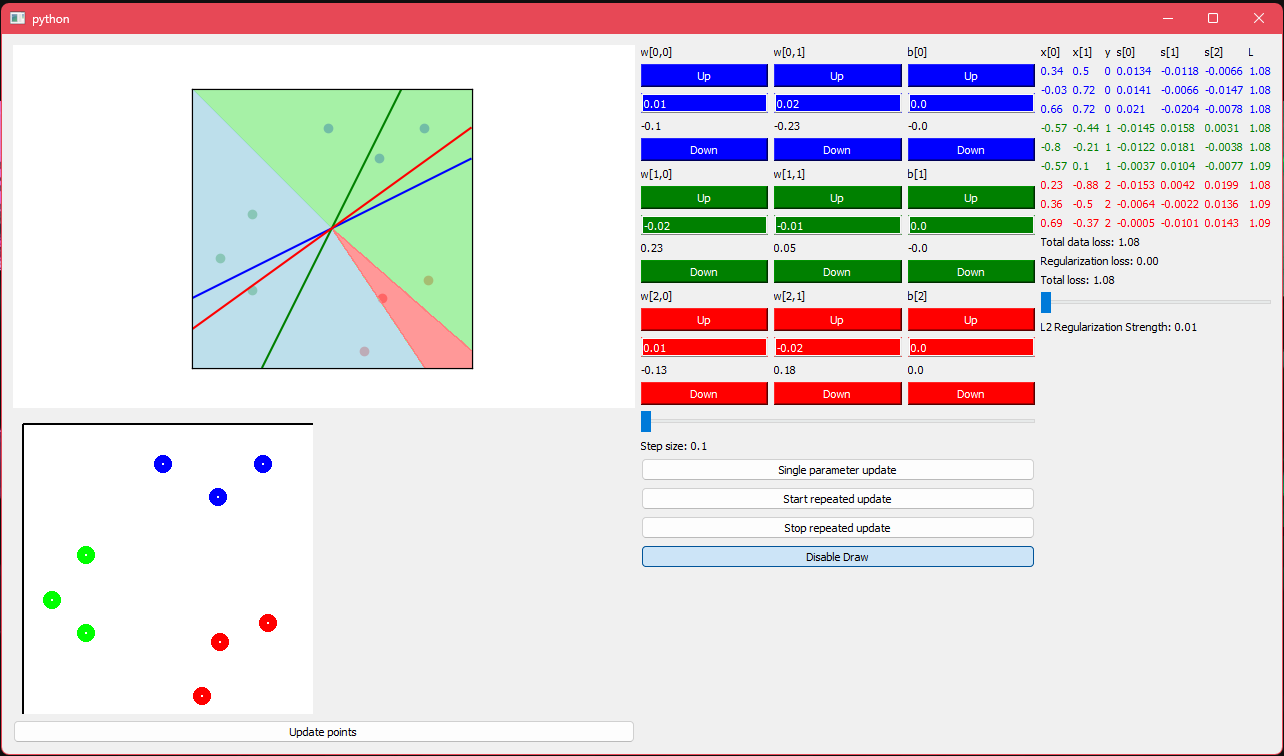
\includegraphics[width=0.4 \columnwidth]{grafics/img-005.png}}
    \hspace{1cm}
    \subfloat[Ejecución de la prueba.\label{fig:6}]{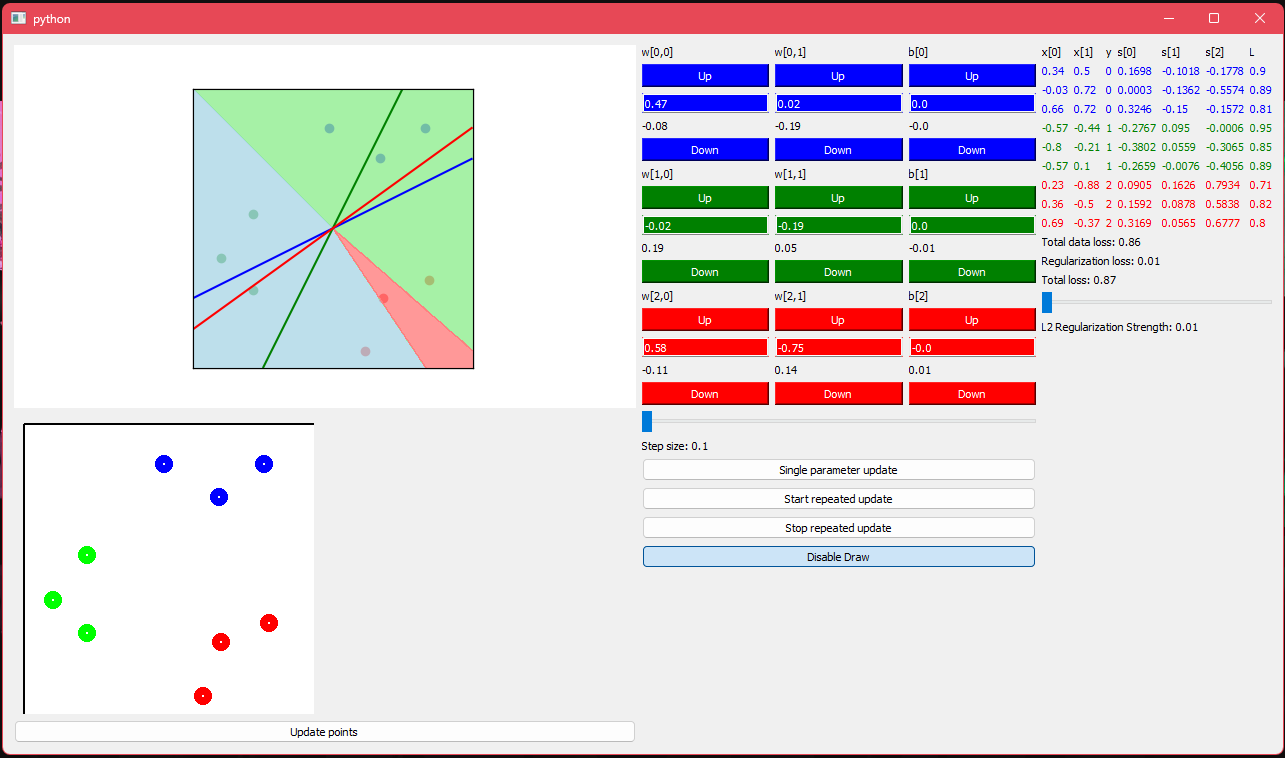
\includegraphics[width=0.4\columnwidth]{grafics/img-006.png}}
    \caption{Figuras 5 y 6}
\end{figure}


En la séptima imagen, mostramos una captura de pantalla de la interfaz de la aplicación después de hacer uso del botón Stop Repeated Update. Esta funcionalidad permite detener todas las actualizaciones periódicas de las métricas, los valores y la gráfica principal, mostrando el resultado actual.

En la imagen, podemos observar que la interfaz ha dejado de actualizarse dinámicamente. Las métricas y los valores se han estabilizado en los resultados obtenidos en el momento en que se detuvo la actualización, y la gráfica principal muestra la clasificación final de los puntos de datos.

Al hacer clic en el botón Stop Repeated Update, se detiene el proceso de actualización repetida y se muestra el resultado actual del modelo de clasificación lineal. Esto permite una evaluación más detallada y precisa de las métricas finales y la clasificación obtenida.

La funcionalidad de detener la actualización repetida con el botón Stop Repeated Update es útil cuando se desea pausar el proceso de actualización continua y analizar el resultado final de la clasificación. Proporciona un punto de referencia para comparar y evaluar el rendimiento del modelo.
%7ma imagen 



En la octava imagen que presentamos en este artículo, mostramos una captura de pantalla de la interfaz de la aplicación después de hacer uso del deslizador Step Size. Esta funcionalidad permite ajustar el tamaño del paso para la actualización de los parámetros, lo que tiene un impacto en la precisión y la velocidad del proceso de clasificación.

Al ajustar el deslizador Step Size, se puede encontrar un balance entre la velocidad y la precisión del proceso de clasificación. Si se establece un valor más grande, los parámetros se actualizarán en pasos más grandes, lo que acelerará el proceso de clasificación pero podría disminuir la precisión. Por otro lado, si se elige un valor más pequeño, los pasos serán más pequeños, lo que podría aumentar la precisión pero llevará más tiempo completar el proceso.

El ajuste del Step Size es crucial para optimizar el rendimiento y la exactitud del modelo de clasificación lineal. Los usuarios pueden experimentar con diferentes configuraciones para encontrar el equilibrio adecuado según las necesidades y los requisitos del problema.
%8va imagen 


%6ta imagen 
\begin{figure}[ht]
    \centering
    \subfloat[Finalización de la prueba.\label{fig:7}]{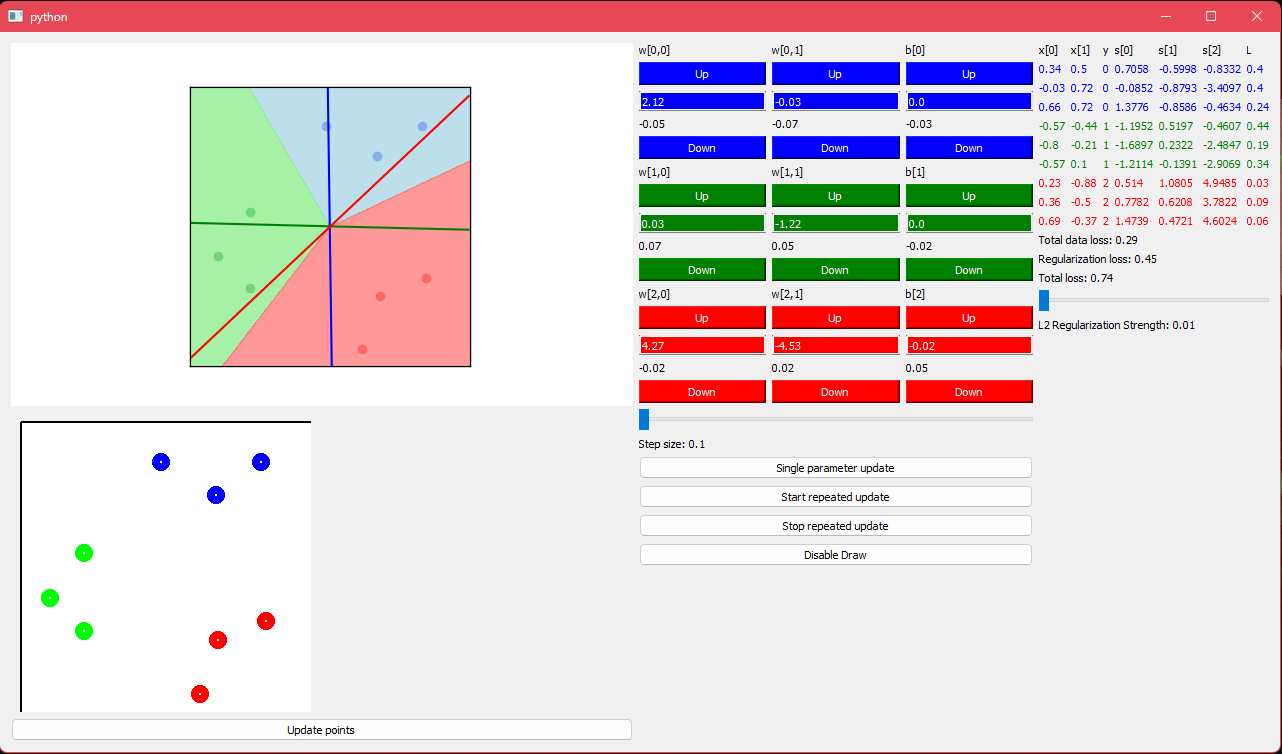
\includegraphics[width=0.4 \columnwidth]{grafics/img-007.png}}
    \hspace{1cm}
    \subfloat[Uso del \textit{step size}.\label{fig:8}]{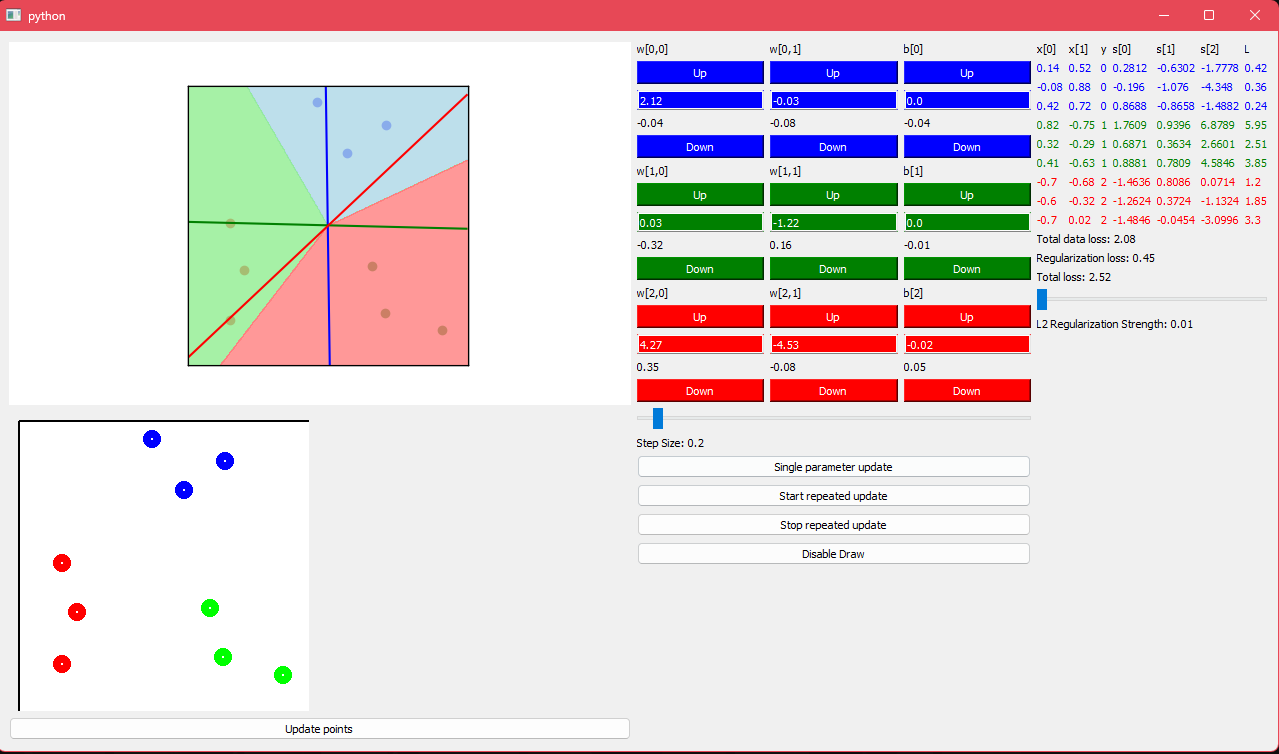
\includegraphics[width=0.4\columnwidth]{grafics/img-008.png}}
    \caption{Figuras 7 y 8}
\end{figure}

En la novena imagen, mostramos una captura de pantalla de la interfaz de la aplicación después de realizar una segunda prueba con la nueva ubicación de puntos y un diferente Step size.

 Las líneas de clasificación y las regiones resultantes se han adaptado a los nuevos datos y parámetros, lo que nos proporciona una visualización actualizada de la capacidad de clasificación del modelo.

 Esta segunda prueba nos permite evaluar cómo los ajustes previos en los parámetros, como el tamaño del paso y otros parámetros relevantes, afectan el rendimiento y la precisión del modelo. Podemos analizar si los cambios en los parámetros han mejorado o afectado la capacidad de clasificación del modelo en comparación con los resultados obtenidos anteriormente.
%9na imagen 



En la décima imagen, mostramos una captura de pantalla de la interfaz de la aplicación después de realizar modificaciones en los pesos utilizando los botones Up y Down. Estos botones permiten ajustar los pesos del modelo de clasificación lineal de manera individual y visualizar el impacto de estos cambios en la clasificación de los datos.

En la imagen, podemos observar que se han realizado modificaciones en los pesos utilizando los botones Up y Down. Cada botón está asociado a un color específico, lo que nos permite identificar rápidamente qué pesos están siendo modificados. Los cambios en los pesos se reflejan en la gráfica principal, donde se muestran las nuevas líneas de clasificación generadas por el modelo.

El botón Up permite aumentar el valor del peso correspondiente, mientras que el botón Down permite disminuirlo. Estas modificaciones proporcionan una forma interactiva de ajustar los pesos y evaluar su impacto en la capacidad de clasificación del modelo.

La visualización en tiempo real de las líneas de clasificación actualizadas nos brinda una comprensión más clara de cómo los cambios en los pesos influyen en la separación de los puntos de datos en diferentes clases. Además, los colores asociados a cada botón facilitan la identificación de los pesos modificados y mejoran la interpretación visual de las modificaciones realizadas.
%10ma imagen 


\begin{figure}[ht]
    \centering
    \subfloat[Ejecución de la segunda prueba.\label{fig:9}]{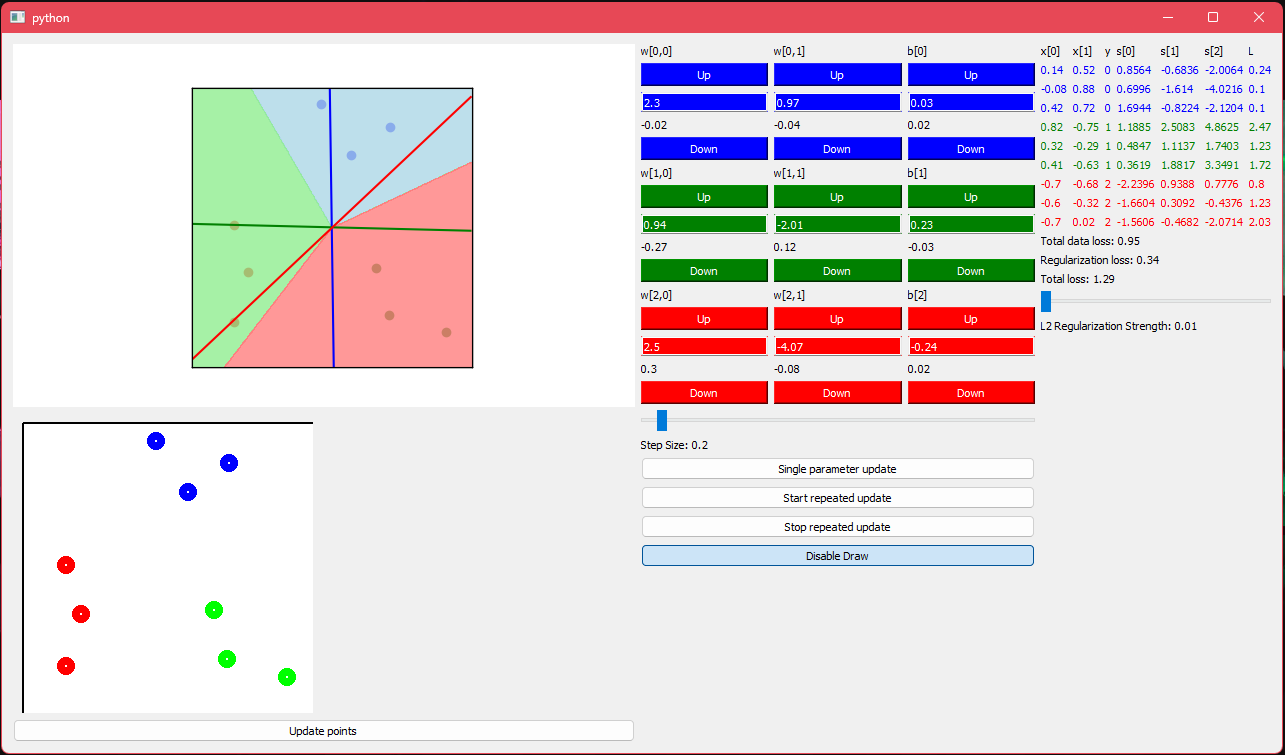
\includegraphics[width=0.4 \columnwidth]{grafics/img-009.png}}
    \hspace{1cm}
    \subfloat[Movimiento de los pesos.\label{fig:10}]{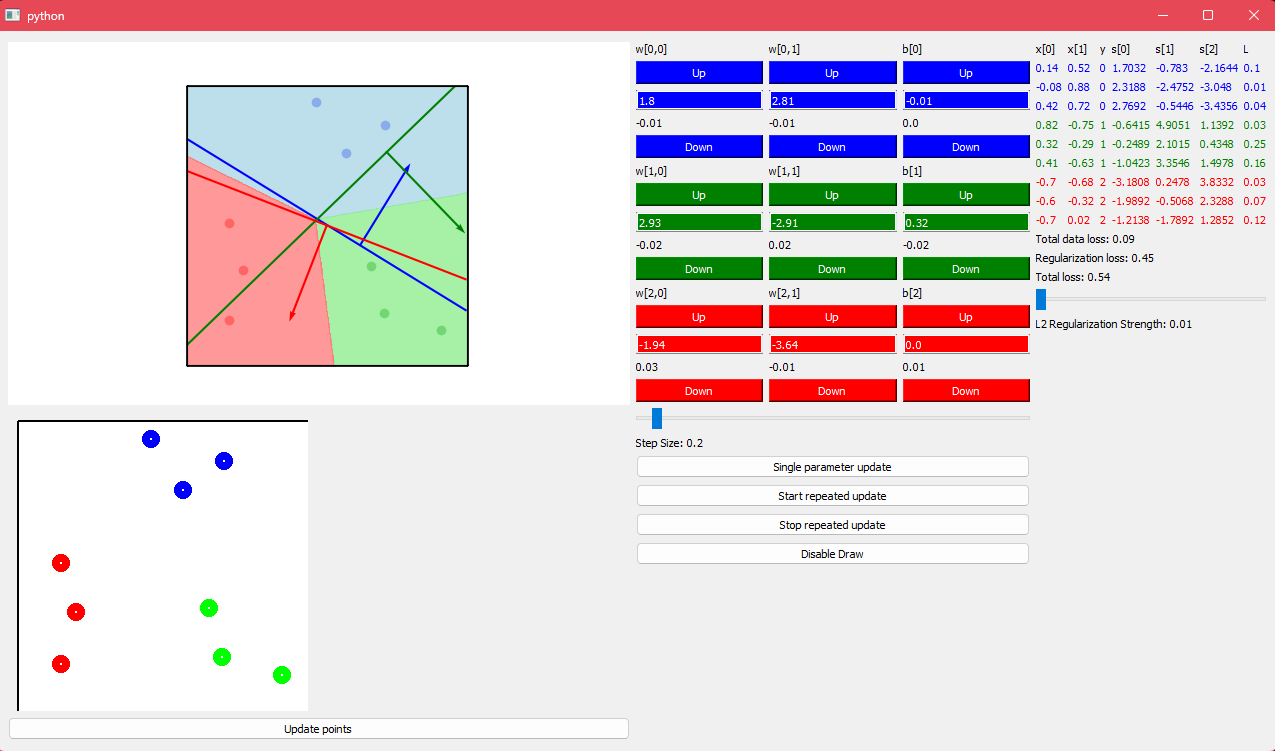
\includegraphics[width=0.4\columnwidth]{grafics/img-011.png}}
    \caption{Figuras 9 y 10}
\end{figure}

En la onceava y última imagen presentada en este artículo, mostramos una captura de pantalla de la interfaz de la aplicación que representa los resultados obtenidos después de completar el proceso de clasificación y evaluación. Esta imagen marca el final del estudio y proporciona una visión general de los resultados alcanzados.

En la imagen, podemos observar los resultados finales del modelo de clasificación lineal, incluyendo las métricas y los valores numéricos relevantes. Estos resultados reflejan la precisión del modelo, la pérdida calculada y otros datos estadísticos asociados.

Además, la gráfica principal muestra la clasificación final de los puntos de datos, con las líneas de clasificación y las regiones determinadas por el modelo. Esta representación visual nos permite apreciar la capacidad del modelo para separar efectivamente los puntos de datos en diferentes clases.

A través de la implementación de este proyecto de investigación, hemos podido analizar y evaluar el rendimiento de los algoritmos de clasificación lineal. Hemos explorado visualmente cómo se produce la clasificación y hemos examinado la influencia de los parámetros en el proceso.
%11va imagen 
\begin{figure}[ht]
    \centering
    \subfloat[Finalización de la prueba.\label{fig:11}]{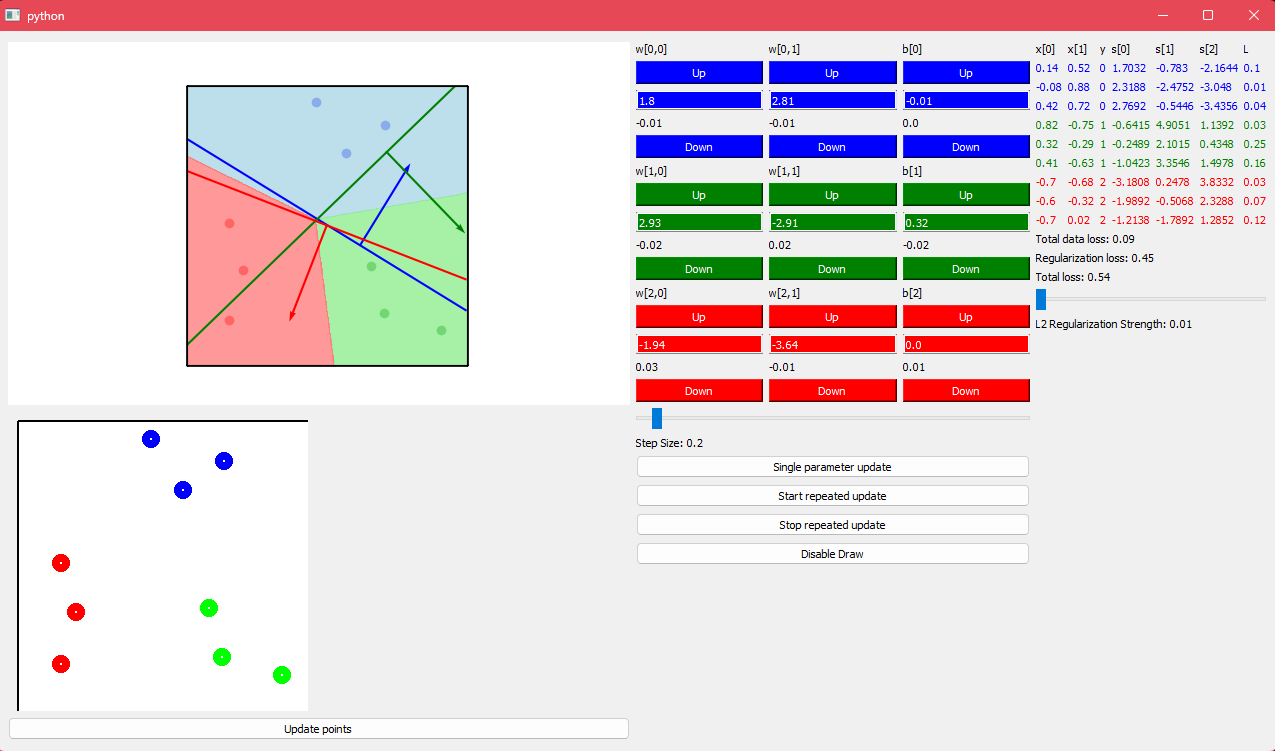
\includegraphics[width=0.4\columnwidth]{grafics/img-011.png}}
    \caption{Figura 11}
\end{figure}






\section{Conclusiones y Trabajo Futuro}

En este trabajo de investigación, hemos realizado un análisis exhaustivo del rendimiento y la visualización de los algoritmos de clasificación lineal a través de la implementación de una aplicación interactiva. Hemos explorado la forma en que se produce la clasificación, evaluado los efectos de los parámetros en el rendimiento del modelo y visualizado la capacidad del modelo para separar los puntos de datos en diferentes clases.

Nuestros resultados demuestran que el modelo de clasificación lineal logra una separación efectiva de los puntos de datos y muestra una mejora en la precisión a medida que se actualizan los parámetros utilizando retropropagación y cálculo de gradientes. La visualización gráfica proporcionada por la interfaz de la aplicación nos ha permitido comprender mejor cómo se adaptan las líneas de clasificación a los cambios en los parámetros y cómo los puntos de datos se clasifican en diferentes regiones.

En cuanto al trabajo futuro, se identificaron áreas de mejora importantes. En primer lugar, es necesario abordar el rendimiento de la aplicación en términos de la velocidad de graficación. Si bien la aplicación ha brindado una visualización efectiva, la optimización del rendimiento permitirá una experiencia más fluida y eficiente para el usuario.

En segundo lugar, se debe investigar cómo el parámetro de Regularization Strength afecta los gradientes y, por lo tanto, el rendimiento del modelo. Una evaluación más profunda de esta relación permitirá ajustar de manera óptima este parámetro y mejorar aún más la capacidad de clasificación del modelo.

Por último, se debe dedicar esfuerzos a mejorar la precisión del clasificador. Esto implica explorar y desarrollar técnicas que permitan una clasificación más precisa y una reducción en los errores de clasificación. Esto podría incluir la exploración de algoritmos más avanzados o el ajuste de los parámetros existentes para mejorar aún más el rendimiento del modelo.




\bigskip

%\noindent {\Large  \textbf{Agradecimientos}}
%Agradecemos a ...


\bibliographystyle{ieeetr}
\bibliography{Bibliografia}
\end{document}

\begin{thebibliography}{14}


\bibitem[Ay74]{Ayoub}
R. Ayoub.
\newblock Euler and the Zeta Fucntion.
\newblock {\em Amer. Math. Monthly}, 81(10):1067--1086, 1974.



\bibitem[Zagier75]{Zagier75}
Don Zagier.
\newblock The first 50 million prime numbers.
\newblock 1975.


\end{thebibliography}


